\section{High Energy Particle Colliders}

The study of high energy particle physics requires laboratory conditions where high densities of energy are concentrated into a miniscule volume.
One method to produce such an environment is with a particle collider.
This section discusses some of the principles that allow colliders to enable the study of otherwise unreachable aspects of our universe.

In general, a collider has the purpose of steering two beams of charged particles such that their constituent particles collide with high energy.
Several subsystems are required to do this.
First, an \emph{accelerator} must boost the beams to high energy with the use of electric fields.
Next, a series of magnets bend and focus the beam. 
A common geometry for a collider, and one employed by the LHC, is a circular arrangement where two counter-rotating beams are guided by dipole magnets around in a circular orbit.
Along the orbit, various magnets will focus and defocus the beam, and alter its trajectory to keep the beam close to a reference orbit.
Finally, the beams are steered to collide with each other in an \emph{interaction point}

% \subsection{Acceleration}
Accelerators are machines designed to accept particles with a given energy and output particles with a higher energy.
A common device to achieve this is the radiofrequency (RF) cavity: a conductive cavity containing an oscillating electric field driven by a periodic potential.
The dimensions of the cavity are selected such that the driving potential produces a resonating standing electromagnetic wave within its volume.
% The standing wave produces an alternating electric field.
A packet of beam particles (a bunch) passing through the cavity will be accelerated by the electric field $\pmb E$, as described by the relativistic Lorentz force in Equation \ref{eqn:lorentzForce}.
\begin{equation}\begin{split}\label{eqn:lorentzForce}
\frac{d\pmb{p}}{dt}=q(\pmb E+\pmb v\cross\pmb B)
\end{split}\end{equation} 
Here $\pmb B$ is the magnetic field and $\pmb v$ is the bunch velocity.
Particles leading or trailing the bunch are pushed back into it.

% \subsection{Magnets}

\begin{figure}[h!]
\captionsetup[subfigure]{position=b}
\centering
\subcaptionbox{Dipole magnetic field\label{fig:magnetsA}}{
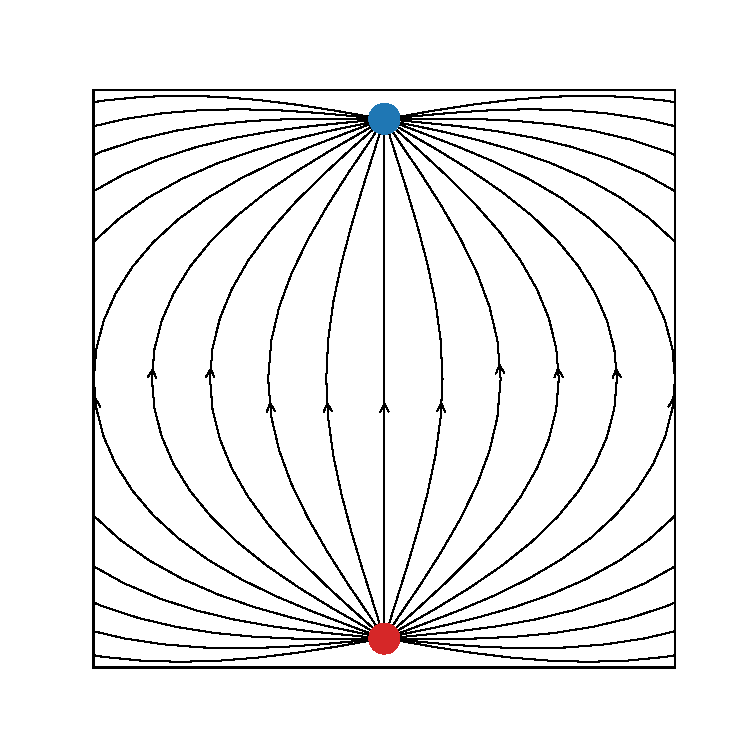
\includegraphics[width=0.3\textwidth]{figures/experiment/lhc/field-1.pdf}
}
\subcaptionbox{Quadrupole magnetic field\label{fig:magnetsB}}{
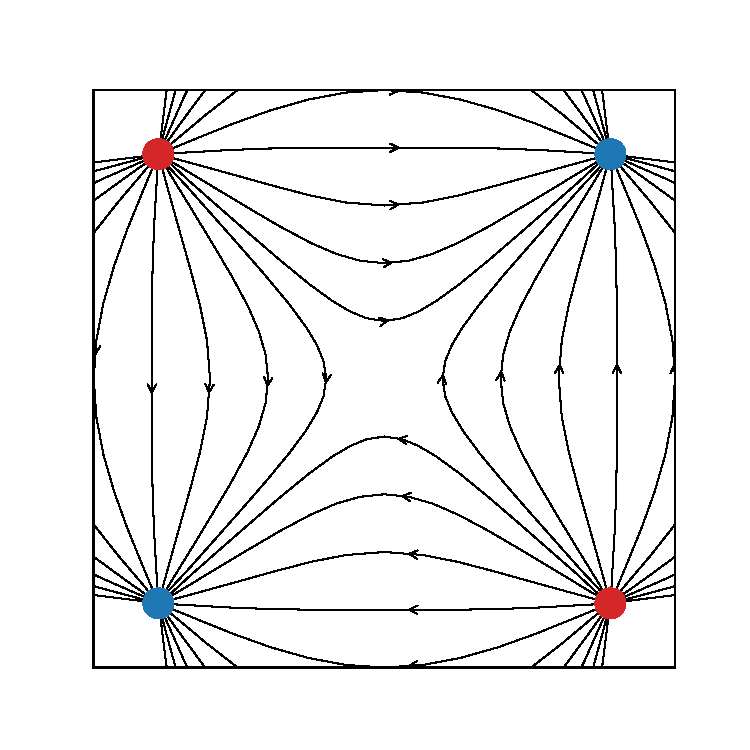
\includegraphics[width=0.3\textwidth]{figures/experiment/lhc/field-2.pdf}
}
\subcaptionbox{Sextupole magnetic field\label{fig:magnetsC}}{
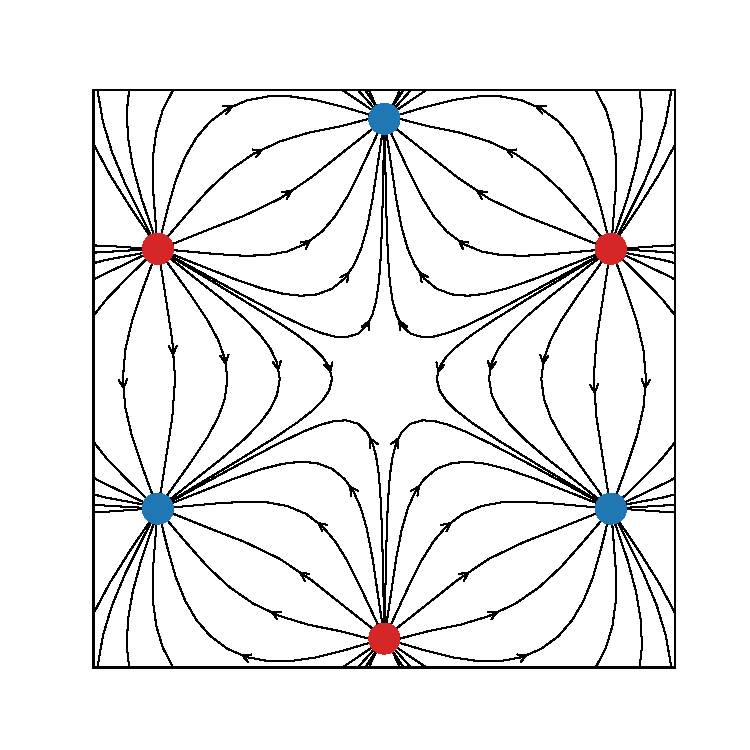
\includegraphics[width=0.3\textwidth]{figures/experiment/lhc/field-3.pdf}
}
\caption{Illustrations of the idealized fields of magnets used commonly in colliders. The poles of fields are shown in red (north) and blue (south). The density of the field lines indicates the strength while the arrows indicate the direction of the magnetic field. In a collider, the fields are orientated such that a particle beam's direction would be into the page.}
\label{fig:magnets}
\end{figure}

A number of magnets are used for a variety of purposes in a collider.
The most prevalent are dipole magnets used to guide the trajectory of the beam around the machine.
Dipole magnets have a nearly uniform magnetic field, $\pmb B$, as illustrated in Figure \ref{fig:magnetsA}
This leads to the circular motion of an incident particle with charge $q$, as described by Equation \ref{eqn:lorentzForce}.

In addition to dipole magnets, quadrupole magnets are used to focus and defocus the beam profile.
An illustration of a quadrupole field is given in Figure \ref{fig:magnetsB}.
A beam passing through a quadrupole is simultaneously focused in one plane and defocused and the perpendicular plane.
Quadrupole magnets are usually grouped in order to provide an overall focusing or defocusing effect on the beam.
A group of two quadrupoles, the second rotated 90 degrees from the first, have the effect of focusing a beam in both planes.

A third magnet configuration is the sextupole, consisting of an arrangement of three dipoles.
A sextupole is useful for adjusting the momentum dependant behavior of the beam. 
This is helpful in maintaining the stability and lifetime of the beam as it circulates the machine.
The field of a sextupole is illustrated in Figure \ref{fig:magnetsC}.

% \subsection{Colliding Beams}
The final task of a collider, after it reaches a stable beam energy, is to steer the beams into collisions.
As the particles making up the beam collide, they interact and transform the incident energy into an explosion of outgoing particles.
The locations of the collisions are such that the outgoing particles can be detected by an experiment.

\section{CERN Accelerator Complex}

\begin{figure}[h!]
\captionsetup[subfigure]{position=b}
\centering
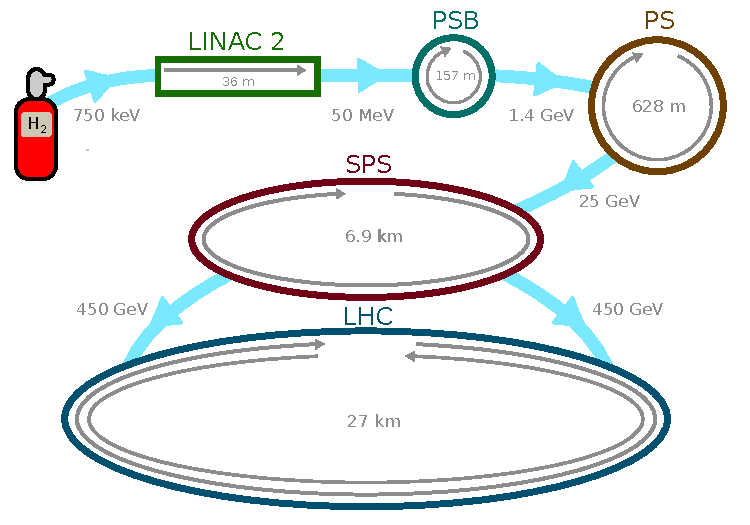
\includegraphics[width=0.8\textwidth]{figures/experiment/cernAccelChain.pdf}
\caption{A schematic view of the path taken by protons through CERN accelerator complex in order to produce beams at the LHC. The energy of the beam is labeled between each accelerator. The length or circumference of the accelerators are labeled, however the beam makes many orbits in each circular accelerator.}
\label{fig:accelComplex}
\end{figure}

The LHC requires input beams with high intensity and energy.
The LHC injector chain is tasked with providing this beam.
Four accelerators make up the chain: the Linac 2, the PS Booster, the PS, and the SPS.
The output of the chain is a proton beam with an energy of 450~GeV.
This section describes each of these machines and the proton beams that they produce \cite{schindl}.
The CERN accelerator complex, as it relates to the production of proton beams, is illustrated in Figure \ref{fig:accelComplex}.

% \subsection{Linac 2}
The first accelerator in the injector chain is the Linac 2.
Protons are sourced from a canister of hydrogen gas and separated by a 90~keV duoplasmatron ion source\footnote{A cathode emits electrons which ionize H$_2$ gas, separating the atoms, which are then accelerated electrostatically towards an anode.}.
The protons enter a 1~m RF quadrupole and are accelerated to 750~keV.
This beam enters the Linac 2, a linear accelerator which dates to 1978.
The Linac 2 accelerates protons to 50~MeV over the course of 36~m using a series of increasingly long RF cavities.

% \subsection{Proton Synchrotron Booster}
The beam output of the Linac 2 is transferred to the first in a series of synchrotrons called the \emph{Proton Synchrotron Booster} (PSB).
Synchrotrons are accelerators where the magnetic field strength is synchronized to the energy of the beam as it accelerates.
The PSB, which began construction in 1968, is a circular synchrotron with a circumference of 157~m.
The incoming beam from the Linac 2 is split vertically by an electrostatic deflector to four levels.
At this stage, the beams are divided into \emph{bunches} of protons, separated by empty space.
These four beams enter four circular rings stacked on top of each other, quadrupling the capacity of the PSB \footnote{The PS is designed to accept five bunches from each PSB ring for a total of 20 bunches. For LHC operation, it accepts one bunch from each PSB ring.} \cite{reich}.
The original PSB was renovated to provide beams for the LHC, and the output energy was increased from 800~MeV to 1.4~GeV. 
This helped reduce instabilities related to producing denser beams.
\cite{schindl}

% \subsection{Proton Synchrotron}
The four beamlines of the PSB are recombined and extracted to the \emph{Proton Synchrotron} (PS)\footnote{Originally named the CERN Proton Synchrotron (CPS).}.
The PS is a circular synchrotron with a circumference of 628~m, four times the circumference of each PSB ring. 
The PS was commissioned in 1959.
Significant effort was undertaken to prepare the PS to supply the beam for the LHC.
This included squeezing four bunches from each PSB ring into one half of the PS and filling the PS with two PSB cycles.
Once the PS has been filled and accelerated its beams to 25~GeV, the spacing between bunches is adjusted to match the LHC's requirements \cite{schindl}.

% \subsection{Super Proton Synchrotron}
The final accelerator before the LHC is the \emph{Super Proton Synchrotron} (SPS).
The SPS was completed in 1976 with a circumference of 6.9~km.
From 1981 to 1990, it provided beams to the UA1 and UA2 experiments, with which UA1 discovered the W and Z bosons.
As with the other CERN accelerators, the SPS underwent upgrades to provide beams to the LHC.
A total of 800 vacuum pumping ports were given Faraday shields to reduce interference caused by the interaction of the beam particles with the wall of the beamline \cite{schindl}.
Two new transfer tunnels were constructed as well to carry the beam from the SPS to ring of the LHC.
These lines carry two beams (clockwise and counter-clockwise) to the LHC, where they are injected into the main rings.
